\section{Adapting Video Diffusion Models to World Models (AVID)} \label{sec:methods}

\subsection{Problem Setting}

In the context of video diffusion models each datapoint is a video, $\mathbf{x} = [x^0, x^1, \ldots, x^{T-1}]$, where $x^\tau$ indicates a video frame. Note that we use superscript indices, $x^\tau$, to indicate steps in time, and subscript indices, $\mathbf{x}_i$, to indicate steps in a diffusion process. We assume that we have access to a pretrained image-to-video diffusion model $\epsilon_{\textnormal{pre}}$, that is trained on web-scale data. Given an initial image, $x^0$, the image-to-video model  $\epsilon_{\textnormal{pre}}$ generates a synthetic video $\hat{\mathbf{x}} = [x^0, \hat{x}^1, \ldots, \hat{x}^{T-1}]$. 

We consider each video to be a sequence of observations generated by a partially observable Markov decision process (POMDP)~\citep{kaelbling1998planning}, with corresponding action sequence $\mathbf{a} = [a^0, a^1, \ldots, a^{T-1}]$. For each domain, we assume access to a dataset of action-labelled videos, $\mathcal{D} = \{(\mathbf{x}, \mathbf{a}), \ldots\}$. Given a new initial image, $x^0$, and action sequence $\mathbf{a}$, the goal is to generate a synthetic video $\hat{\mathbf{x}}$ that accurately depicts the ground-truth realization of the actions.

To utilize the pretrained model $\epsilon_{\textnormal{pre}}$, we need to add action-conditioning to the model as accurate videos cannot be generated without the actions. Adding a new conditioning signal to a pretrained diffusion model is well-explored in previous works~\citep{zhang2023adding, mou2024t2i,mokady2023null}. However, most existing works assume access to the parameters of the pretrained model. In this work, we assume that we \textit{do not have access to the parameters of the pretrained model}.


\subsection{Limitations of naive adaptation of \cite{yang2024probabilistic}}
\label{sec:yang_limitations}

\cite{yang2024probabilistic} propose to adapt a pretrained diffusion model to a specific use-case without access it its weights by composing (omitting the prior strength $\lambda$):
%
\begin{align}
\mathbf{\epsilon}_{\text{PoE}} (\mathbf{x}_i, i, c) := 
\mathbf{\epsilon}_{\text{pre}} (\mathbf{x}_i, i, c) + \mathbf{\epsilon}_{\text{adapt}} (\mathbf{x}_i, i, c) \label{eq: yang}
\end{align}
However, this method has a fundamental limitation that it will produce biased samples. To see this, consider the following forward diffusion process 
$$d\mathbf{x} = -\frac{1}{2} \beta(t) \mathbf{x} dt + \sqrt{\beta(t)} dW, $$
where $t$ indicates continuous time. Assume the intial target distribution at $t=0$ is $p_0(\mathbf{x}) := p_\textnormal{PoE} = \frac{p_{\text{pre}}(\mathbf{x})p_{\text{adapt}}(\mathbf{x})}{Z}$. 
%
Notice that the transition kernel can be written as \citep{sarkka2019applied}:
$$p(\mathbf{x}_t|\mathbf{x}_0) = \mathcal{N}(\mathbf{x}_t; \mathbf{x}_0 e^{-\frac{1}{2} \int_0^t \beta(s) ds }, I-I e^{- \int_0^t \beta(s) ds})$$
Therefore, for $\forall t>0$, the resulting distribution is the convolution $p_t(\mathbf{x}_t) = p_0(\mathbf{x}_0) * \mathcal{N}(\mathbf{x}_t - \mathbf{x}_0 e^{-\frac{1}{2} \int_0^t \beta(s) ds }; 0, I-I e^{- \int_0^t \beta(s) ds})$. 
%which does not factorize into a PoE of $p_{t, \text{pre}}$ 
%and $p_{t, \text{adapt}}$ distributions anymore. As a result
%and the corresponding score function $s_t(\mathbf{x}_t)$ is given by: $$s(\mathbf{x}_t, t) = \nabla_{\mathbf{x}_t} \log \left [p_0(\mathbf{x}_0) * \mathcal{N}(\mathbf{x}_t - \mathbf{x}_0 e^{-\frac{1}{2} \int_0^t \beta(s) ds }; 0, I-I e^{- \int_0^t \beta(s) ds}) \right ].$$
%
Due to the fact that convolution does not distribute over multiplication, the resulting score $s(\mathbf{x}_t, t)$ cannot be expressed as a sum of the two individual score functions:
\begin{align*}
s(\mathbf{x}_t, t)  = & \nabla_{\mathbf{x}_t} \log \left [p_0(\mathbf{x}_0) * \mathcal{N}(\mathbf{x}_t - \mathbf{x}_0 e^{-\frac{1}{2} \int_0^t \beta(s) ds }; 0, I-I e^{- \int_0^t \beta(s) ds}) \right ] \\
 \neq  & \nabla_{\mathbf{x}_t} \log \left [ p_{0, \text{pre}}(\mathbf{x}_0) * \mathcal{N}(\mathbf{x}_t - \mathbf{x}_0 e^{-\frac{1}{2} \int_0^t \beta(s) ds }; 0, I-I e^{- \int_0^t \beta(s) ds}) \right ] \\
& + \nabla_{\mathbf{x}_t} \log \left [ p_{0, \text{adapt}}(\mathbf{x}_0) * \mathcal{N}(\mathbf{x}_t - \mathbf{x}_0 e^{-\frac{1}{2} \int_0^t \beta(s) ds }; 0, I-I e^{- \int_0^t \beta(s) ds}) \right ]
\end{align*}
As a result, the true noise prediction of the target distribution also cannot be expressed as a sum: $\mathbf{\epsilon}_{\text{PoE}} (\mathbf{x}_t, t, c) \neq
\mathbf{\epsilon}_{\text{pre}} (\mathbf{x}_t, t, c) + \mathbf{\epsilon}_{\text{adapt}} (\mathbf{x}_t, t, c)$. Therefore, the composition in  \Cref{eq: yang} does not hold and  will result in biased samples. 
%
In the following section, we propose AVID to overcome this limitation.
%
Rather than attempting to compose two independently trained models, AVID uses the outputs of the pretrained model to train an adapter that directly optimizes the denoising loss.
% 
% \mathbf{\epsilon}_{\text{PoE}} (\mathbf{x}_t, t, c) & \propto \nabla_{x_t} \log \left [p_0(\mathbf{x}_0) * \mathcal{N}(\mathbf{x}_t - \mathbf{x}_0 e^{-\frac{1}{2} \int_0^t \beta(s) ds }; 0, I-I e^{- \int_0^t \beta(s) ds}) \right ]\\ 
% & \neq  \nabla_{\mathbf{x}_t}  \log \left [p_{0, \text{pre}}(\mathbf{x}_0) * \mathcal{N}(x_t - x_0 e^{-\frac{1}{2} \int_0^t \beta(s) ds }; 0, I-I e^{- \int_0^t \beta(s) ds}) \right ]\\
% & +  \nabla_{\mathbf{x}_t} \log \left [ p_{0, \text{adapt}}(\mathbf{x}_0) * \mathcal{N}(\mathbf{x}_t - \mathbf{x}_0 e^{-\frac{1}{2} \int_0^t \beta(s) ds }; 0, I-I e^{- \int_0^t \beta(s) ds}) \right ]
% %& = \boldsymbol{\epsilon}_{\textnormal{adapt}}(\mathbf{x}_i, \mathbf{a}, i, x_0) +  \boldsymbol{\epsilon}_{\textnormal{pre}}(\mathbf{x}_i, i, x_0).
% \end{align*}
% Therefore, the composition \Cref{eq: yang}  does not exactly hold and will result in biased samples. 
%In fact, this is a fundamental limitation of diffusion models and we theoretically show (TODO: in appendix) that there does not exist a forward SDE process that preserves \Cref{eq: yang}. 

\subsection{Adapting Video Diffusion Models to World Models (AVID)}
\label{sec:avid}
AVID is a new approach for diffusion model adaptation that does not require access to the pretrained model.  The motivation for AVID is that while pretrained image-to-video models can generate \textit{realistic} videos, they cannot generate videos that are \textit{accurate} with respect to a given sequence of actions. To achieve accuracy, the pretrained model must be guided towards the correct generation for the action sequence. However, as our experiments show, techniques such as classifier(-free) guidance do not perform well in this setting. AVID addresses this by training a lightweight adapter to adjust the output of the pretrained model to achieve accurate action-conditioned video predictions.




\begin{figure}[t]
    \centering
    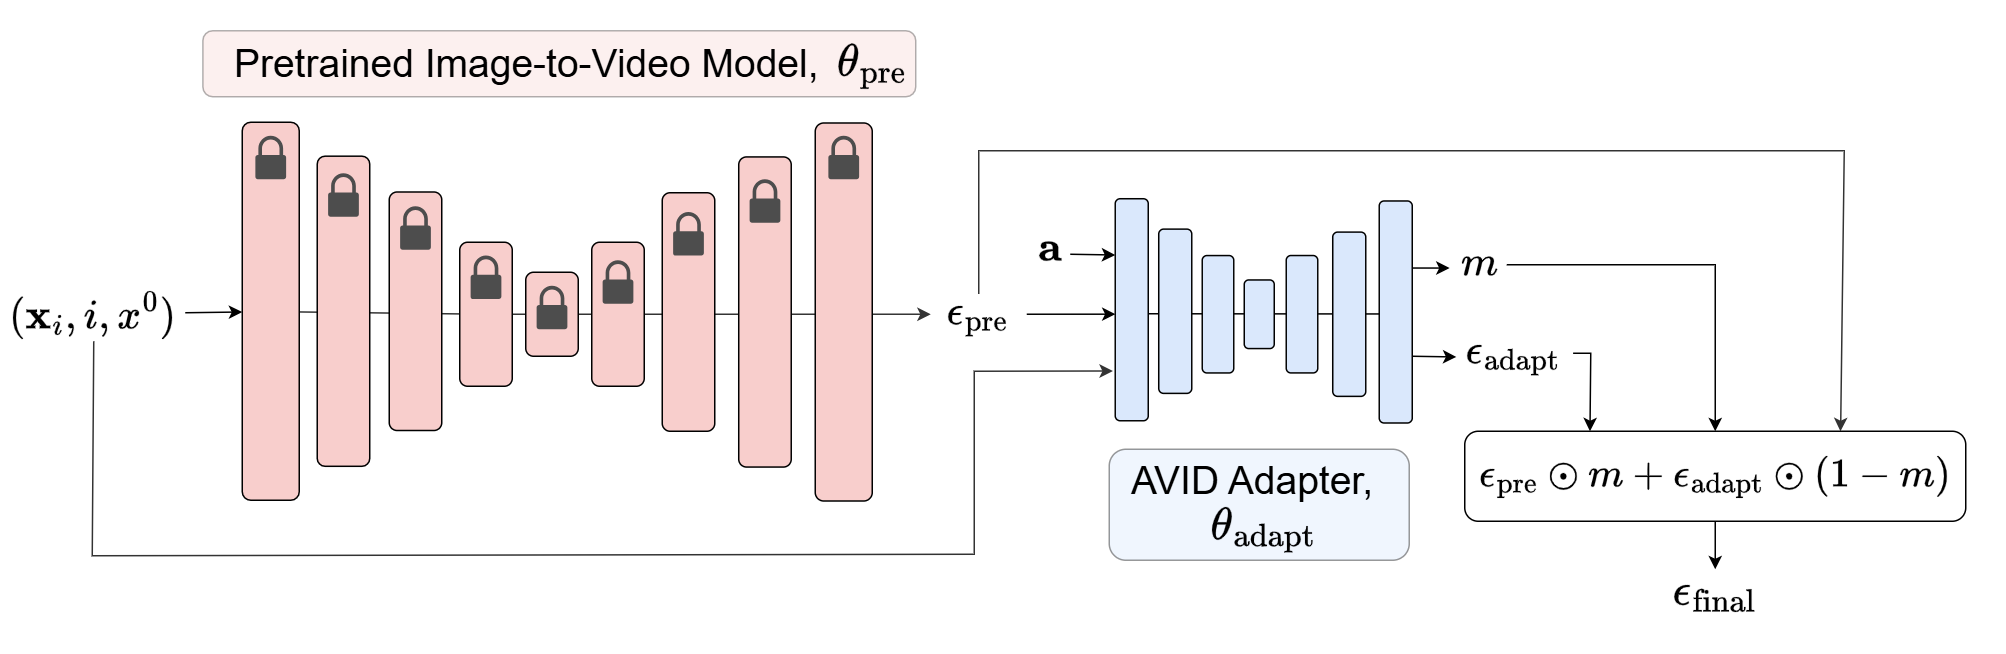
\includegraphics[width=\linewidth]{figures/video-adapter.png}
    \caption{Overview of AVID world model adapter architecture.}
    \label{fig:your_label}
\end{figure}
AVID trains an adapter that takes the output of the pretrained model as an input. AVID learns to generate a mask, and uses this mask to combine the outputs of the pretrained model with those of the adapter. The final combined output is used to compute the standard denoising loss, and the adapter parameters are trained to optimize this loss. 
We train the AVID adapter using samples $(\mathbf{x}, \mathbf{a})$ from the action-labelled dataset.
%
For the pretrained image-to-video model $\epsilon_{\textnormal{pre}}$ we assume that we do not have to access to it's parameters, $\theta_{\textnormal{pre}}$, but we can run inference using the model to obtain it's noise predictions.  To do this, we input a noisy video, $\mathbf{x}_i \in \mathbb{R}^{T \times h \times w \times c}$, initial image, $x^0 \in \mathbb{R}^{h \times w \times c}$, and diffusion step, $i$, to the pretrained image-to-video model to obtain its noise prediction, $\epsilon_{\textnormal{pre}}(\mathbf{x}_i, i, x_0) \in \mathbb{R}^{T \times h \times w \times c}$. The parameters of the pretrained model $\epsilon_{\textnormal{pre}}$ are not modified.

The adapter that we train is a 3D UNet~\citep{ho2022video, ronneberger2015u} consisting of a sequence of spatio-temporal blocks with residual connections. Each spatio-temporal block consists of a 3D convolution, spatial attention, and temporal attention~\citep{ho2022video}. The UNet takes as input a tensor of shape $\mathbb{R}^{T \times h \times w \times 3c}$. The input consists of the noisy video, $\mathbf{x}_i $, the output of the pretrained model, $\epsilon_{\textnormal{pre}}(\mathbf{x}_i, i, x_0)$, and the initial image $x^0$ repeated $T$ times across the time dimension. These three inputs are concatenated channel-wise to create the input tensor.

The adapter is also conditioned on the diffusion step $i$ and the sequence of actions $\mathbf{a}$. For noisy video $\mathbf{x}_i$ we embed the diffusion timestep according to a learned embedding table to get the diffusion step embedding $e_i$. For each timestep $\tau$ of the noisy video $\mathbf{x}_i$ we embed the corresponding action $a^\tau$ to compute the action embedding $e_{a}^\tau$ using an embedding table for discrete actions or a linear layer for continuous actions. In each block, these two embeddings are concatenated and processed by an MLP to compute the scale and shift parameters, $\gamma^\tau$ and $\beta^\tau$, for the $\tau^{th}$ frame. These parameters scale and shift the feature maps of the $\tau^{th}$ frame after each 3D convolution~\citep{perez2018film}.


To inject the correct action-conditioning into the predictions made by the pretrained model, the adapter needs to erase incorrect motions predicted by the pretrained model and add the correct motion. To facilitate this, the adapter outputs a tensor of shape $\mathbb{R}^{T \times h \times w \times (c + 1)}$ consisting of a mask, $m \in \mathbb{R}^{T \times h \times w \times 1}$ which is bounded between 0 and 1 by a sigmoid layer, and the noise prediction from the adapter $\epsilon_{\textnormal{adapt}}$.
%
The mask is then used to combine the noise predictions from the pretrained model and the adapter according to:
\begin{equation}
    \epsilon_{\textnormal{final}}(\mathbf{x}_i, \mathbf{a}, i, x_0) = \epsilon_{\textnormal{pre}} \odot m + \epsilon_{\textnormal{adapt}} \odot (1 - m), 
\end{equation}
where $\odot$ denotes the Hadamard product, and the mask is broadcast across all $c$ channels.
%
The parameters of the adapter model, $\theta_{\textnormal{adapt}}$, are optimized to minimise the standard unweighted denoising loss using $\epsilon_{\textnormal{final}}$:
\begin{equation}
    \mathcal{L}(\theta_{\textnormal{adapt}}) = \mathbb{E}_{(\mathbf{x}, \mathbf{a}) \sim \mathcal{D}, {\boldsymbol\epsilon \sim \mathcal{N}(\mathbf{0}, \mathbf{I})}, i \sim \mathcal{U}(\{1, 2, \dots, N\})}\|\epsilon_{\textnormal{final}}(\mathbf{x}_i, \mathbf{a}, i, x_0) - \boldsymbol\epsilon \|^2.  \label{eq:adapt_loss}
\end{equation}
In the case where $\epsilon_{\textnormal{pre}}$ is a latent diffusion model, we assume that we can also run inference on the corresponding encoder and decoder.
%
For each training example, we first encode the video: $\mathbf{z} = \mathtt{enc}(\mathbf{x})$ where $\mathbf{z} \in \mathbb{R}^{T \times h' \times w' \times c'}$, and add noise to this latent representation of the video to produce noisy latent $\mathbf{z}_i$.
%
The rest of the pipeline proceeds in the same manner, except that the initial image $x^0$ is replaced by  the latent corresponding to the first frame, $z^0$, and the noisy video $\mathbf{x}_i$ is replaced by the noisy latent $\mathbf{z}_i$. The adapter loss in Equation~\ref{eq:adapt_loss} predicts the noise added to the latent sample, and we decode the sampled latent to generate the final video.

